\documentclass[12pt]{article}

%\usepackage{times} %for Times New Roman, if required
\usepackage[top=1in, bottom=1in, left=1in, right=1in]{geometry} %adjust margins. TODO: hack to fix large top margin
\usepackage{setspace} %allows doublespacing, onehalfspacing, singlespacing
\usepackage{enumitem} %for continuing lists
\usepackage{titling} %for moving the title
\usepackage[normalem]{ulem} %for underlining
\usepackage{graphicx}

%redefine section numbering to match Mayron's style
\renewcommand{\thesection}{\arabic{section}} %make sections use numbers
\renewcommand{\thesubsection}{\alph{subsection}} %make subsections use letters
\renewcommand{\thesubsubsection}{\roman{subsubsection}} %subsubsections use romans

\setcounter{tocdepth}{2}

\begin{document}

\begin{spacing}{.4}
\setlength{\droptitle}{-7em}
\title{CSE 485 Semester Report \\  Team 1, Friday 10:30am}
\author{Connor Alfheim \and Ryan Dougherty \and David Ganey \and Dylan Lusi \and Joseph North \and Ben Roos}
\maketitle
\end{spacing}

\begin{spacing}{1.5}
\noindent
Project sponsors: Dr. Judd Bowman and Dr. Danny Jacobs \\
Project description: A virtual observatory for the Murchison Widefield Array radio telescope.
\newpage

\tableofcontents
\newpage

\section{Executive Summary}
The Murchison Widefield Array (MWA) is an enormous radio telescope in Australia used by scientists to monitor hydrogen radiation. This telescope assists scientists interested in learning about the formation of the universe. EoRLive, a website which allows scientists to browse the data collected by the MWA, is in need of additional functionality. This project was formed to enhance the current EoRLive website and to allow the scientists who use it to engage with their data more efficiently.
\\ \\
This semester, we worked with our sponsors to understand the project's requirements and came up with an architecture containing three fundamental layers: a database layer, a logic layer, and a user interface layer. Our primary deliverable for the semester was a prototype that involves all three layers. We developed it to gain an understanding of the technologies and challenges associated with the different components of the project. The prototype is a range-based data browser that enables users to view specific observation data sets. Our plan for the second semester is to implement the project's key features and integrate them into the full site.

\section{Introduction}
\subsection{Project description}
This semester, we produced a website that functions as a range-based data browser for the MWA telescope's observations. It has user accounts and offers the user the ability to select a custom date range. The site displays a list of observations made by the telescope in that date range, and an interactive graph that shows the status of the telescope's data pipeline in that date range, from scheduling the observations to transferring the observation data to a database at MIT.
\subsection{Purpose of project}
The motivation for this project was to make improvements upon the existing site, which lacked some key features the MWA researchers really wanted. They wanted a site that would allow them to monitor the status of the telescope in real time, annotate and share data sets, create conversations about the data through forum-style discussions, and write custom queries that allow them to see the data they want, all on an intuitive Web platform. Ultimately, the goal for this project was to build a more dynamic, collaboration-focused, and customizable site. It will allow the scientists to focus more on their research and less on the tools that connect them to their data.

\section{Scope}
\subsection{Original Definition}
The original scope definition was to develop a website based on a user interface mockup that was provided in a document given to us by our project sponsors, and to proceed with implementation on a feature-by-feature basis. The document specified a visual view of the telescope array, user account support, and inter-user interaction functionality. We also included desired features that were not present in the provided mockup, such as annotating and sharing data sets.

\subsection{Change of scope and reason for change}
Shortly after commencing work on our project's implementation, we stalled. We realized that scoping our project solely in terms of large, complex features didn't give us any good places to start because just thinking about features didn't offer much detail as to the implementation specifics. We met with our project sponsors and decided to modify the scope by dividing it into three distinct ``layers", which allowed us to break the features down into smaller and more manageable components.
\\ \\
The lowest layer is the actual telescope data itself. As explained to us by our project sponsors, the main component of the website will be displaying the data---our goal for this layer is to pull the telescope data out of the databases in a meaningful way.
\\ \\
The middle layer is the logic layer, which will be the layer in-between the user interface and data layers. There is not a well-defined API for extracting the data from the databases---our team will have to develop an API with demos/documents/plots, and more---so that others can extend the functionality later. Also, the databases are extremely complex, so we need to develop an object-relational mapping (ORM) for modeling the data. 
\\ \\
The third layer is the user interface. There are several features that need to be added---one is user accounts. Users need to be able to register and log in to the website. Another important feature is commenting---we need to allow users to leave comments on data sets, enabling conversations between users. There will also be direct links to data sets that users can share in their discussions. The project sponsors also wanted more interactivity in the website, such as manually flagging data streams, seeing which users are also online (possibly to start a conversation), displaying an interactive diagram of the array, and more.

\subsection{Use case diagram}
\subsubsection{Figure 1: User with account}
\begin{center}
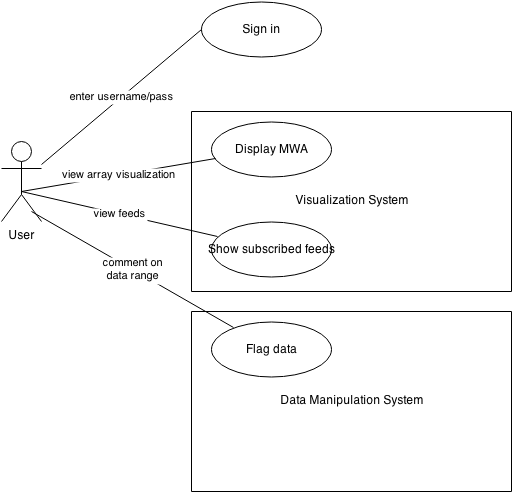
\includegraphics{usecase1} %we can use this to insert .png files in the same directory
\end{center}
\newpage
Users who are not logged in are not permitted to edit the data:
\subsubsection{Figure 2: User without account}
\begin{center}
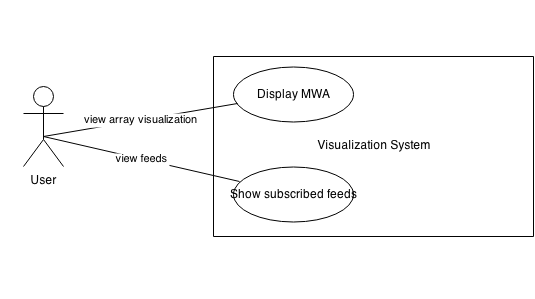
\includegraphics{usecase2}
\end{center}

\subsection{Description of actors}
In the figures above, the actors are viewers of the EoRLive website. The users in Figure 1 are all scientists, and must have been approved by a site admin in order to view the website. The actor in Figure 2 encompasses any user, regardless of affiliation with a specific scientific organization. 

\subsection{User stories}
\begin{enumerate}
\item User views website
	\begin{itemize}
		\item As a user who is not signed in, I want to see a graphical representation of the Murchison Widefield Array so I can tell whether any of the telescope's nodes are malfunctioning.
		\item Given that the data stream is valid, when the user loads the page, the page should show a graphic that shows the state of the array.
	\end{itemize}
\item User signs in
	\begin{itemize}
        		\item As as user with an account, I want to sign in with my account on the site so I can view the site with my custom settings enabled.
        		\item Given that the user's credentials are valid, the website should allow the user to sign in and should load their personal settings before rendering the page.
		\item Given that the user's credentials are invalid, the website should refuse to allow the user to sign in but should still show the status of the array.
	\end{itemize}
\item User modifies settings
	\begin{itemize}
		\item As a signed-in user, I want to modify my subscription settings so I can choose which data streams I will be shown.
		\item Given that the user is signed in, the user should be permitted to modify subscription settings.
		\item Given that the user is not signed in, the user should not be permitted to see or modify subscription settings.
	\end{itemize}
\item User flags data
	\begin{itemize}
		\item As a signed-in user, I want to leave comments on data streams so I can collaborate with other users and generate discussions about the data.
		\item Given that the user is signed in, and that the data stream is valid, the user should be permitted to leave comments on a data stream.
		\item Given that the user is not signed in or that the data stream is not valid, the user should not be permitted to leave comments on that data stream.
	\end{itemize}
\end{enumerate}

\section{Project Plan}
\subsection{First semester}
For the first semester, one goal of the project was to identify and refine the most useful features which could realistically be implemented by the end of the year in order to establish the requirements for a successful product. Another goal was to develop a prototype of the website that involved the three layers determined in our project scope and demonstrated several of the features that would be implemented more fully in the second semester. Specifically, we aimed to implement the ability to select a range of dates to restrict the data that would be displayed on the main page, and the ability to associate information with a user profile, such as comments and saved data ranges. The final goal was to familiarize ourselves with the development tools we would be using so that the team could progress more quickly on subsequent work.
\subsection{Second semester}
For the second semester, the goal of the project is to port the improvements made to the prototype to the full site. Additional features will be added to create version three of the EoRLive website. A visual representation of the telescope will help scientists monitor its health. User communication functionality will help scientists collaborate more effectively and discuss data in new ways. For example, the ability to generate hyperlinks to specific data ranges will allow for quick sharing of information. Additionally, the team will work to maintain extensibility on the website by providing an API through which scientists can create additional plots and views for new types of data streams. These four new features (a telescope monitor, user forum style communication, hyperlinks to data ranges, and extended plotting capabilities) define the backbone of the second semester development effort, though additional functionality may be added as well if time permits.

\section{Development Approach}
 While the team spent longer in the requirements and design phase than the normal agile process, we used agile development methods to create our prototype. During the first few weeks of the semester, our team fell into the same trap that occurs to many waterfall projects: we were overly focused on documentation and gathering of requirements at the expense of producing usable software. During this time, each new idea from us or our sponsor changed our potential design. After multiple weeks of working through design decisions and restructuring the design of our product, we moved to an agile methodology to produce a usable product. 
\\ \\
Once we adopted agile development, our focus changed from producing a fully functional website to creating a core site with extensible code that can be later changed to add additional features. Our reasoning for adopting an agile process was that we wanted to quickly produce a usable site that our sponsors could use and provide feedback for. From the core site, our sponsors and we were able to identify the current features that need refinement and the next set of features that need to be implemented. 


\section{Design Overview and Decisions}
\subsection{Modularity}
For the prototype, each feature was programmed to be a separate module from the other features. This design allows for highly reusable code as the same item on different pages does not become duplicated code. For instance, our header at the top of the page is located in one HTML template that our other templates simply extend, allowing us to reuse it all over the site. Our team only needs to modify one file in order to change the layout of the site. Additionally, visual components such as tables and graphs are implemented as their own templates that are constructed on the backend and simply injected into the page so they can be easily swapped in and out. In addition, this design could aid in the implementation of subscription feeds later---users could customize which views of the data they have by subscribing to different modules.

\subsection{Database}
Our prototype's database is managed by SQLite, since it is easier to set up than a more robust server-side relational database management system such as PostgreSQL. This database contains all of the custom site information like user information, comments, and data ranges that users save.
\\ \\
In addition to the site specific data, the database stores consolidated information from the many outside databases that contain the data relevant to this project. The data from the telescope are stored in multiple remote databases. The data germane to this project is a small subset of the total data and needs to be combined from the multiple databases. A query to select and join the relevant data from the many databases has too long of a response time for a positive user experience. To fix this slow consolidation of data, we wrote a script that imports the newest data every few minutes. Once the data is processed and stored locally, the site can deliver the proper content quickly.

\section{Technology and Tools}
\subsection{Programming Languages}
The development for this website uses many of the standard web-development languages. Front-end design is accomplished using HTML and CSS. Some client-side code is run with JavaScript, though this is minimal. The primary server-side language used is Python, in conjunction with a Web application framework called Flask.  Given that many members of the scientific community, who are the targeted users of our application, are proficient in Python, and that one of the goals of the project is to allow users to import custom data modules via scripts, a Python framework such as Flask seemed to be the obvious choice.  Finally, we use SQL in our scripts that run regularly to pull data from the MIT databases.

\subsection{Other Tools}
The development environment used by the team is managed by Vagrant. Vagrant is an open-source tool that allows teams to create specific virtual machines, allowing everyone to develop on their own computers but in environments with identical configurations. This allows team members to focus on the code rather than problems related to their specific configuration, which can be an issue with Web development when developers must run Web servers with many dependencies locally.  A Vagrant machine was provided to us by our sponsors as the means to run a virtual machine equivalent in functionality to the EC2 server hosting the current version of the EoRLive website.
\\ \\
The version control tool chosen to manage our codebase is Git, with GitHub as a host and collaborative tool. Comments and issues on GitHub allow the team to communicate directly on the code. Slack, a team communication tool, was used to keep the development team connected. Standard email communication was used in conjunction with meetings to communicate with the sponsors.

\section{Preliminary Results}
Our primary deliverable for this semester is a small website that allows the user to browse data based on date ranges. It includes support for user accounts, which are added via the command line on the server. The user logs in with their username and password and is taken to the main screen that contains "Start" and "End" datetime selectors that are filled in with reasonable default values (the end time is the current UTC time and the start time is 24 hours prior). Clicking the "Get observations" button loads a table below that displays a list of telescope observations that occurred in that range (or are scheduled in that range, if the range extends into the future). Specifically, each entry in the table includes the observation's ID, name, and who scheduled the observation. Below this table is a graph that displays the status of the telescope's data pipeline during that range. Specifically, it is a line graph that shows the total observation hours scheduled for the telescope versus how many hours have actually been observed, and how many hours' worth of observation data have been transferred from the telescope to databases at MIT. The graph is interactive; the user can toggle the data sets in the legend to choose which ones are shown in the graph.
\\ \\
We demonstrated our prototype to our sponsor, Dr. Jacobs, and received some useful feedback. While the telescope observation table was purposeful in that it showed we were interacting with the telescope data, it isn't that useful to a user of the site. Instead, we should use the same data and display it in a more meaningful way, perhaps as a histogram showing how many observations have happened on each day. Additionally, the graphs we have on the site should be more interactive; specifically, the user should be able to make range selections on the graphs themselves to choose the data they see rather than having to rely on the controls at the top of the page. This would create a more natural connection between the user and the data presented to them on the page, since they could interact with it visually. Finally, the main data page should be capable of being linked to by a unique URL that allows users to access the same data range. Users should be able to save these links to their account so they can easily share them with others.

\subsection{Figure 3: The login page}
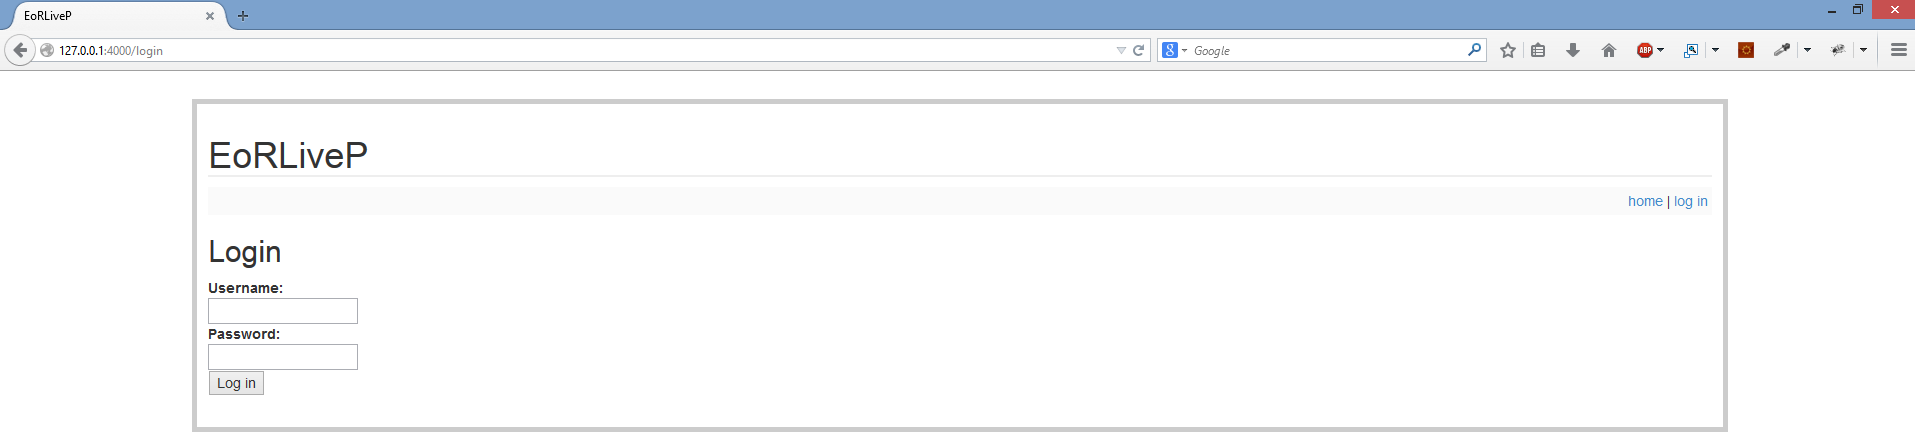
\includegraphics[width=\textwidth]{screenshot1}

\subsection{Figure 4: The data browsing page}
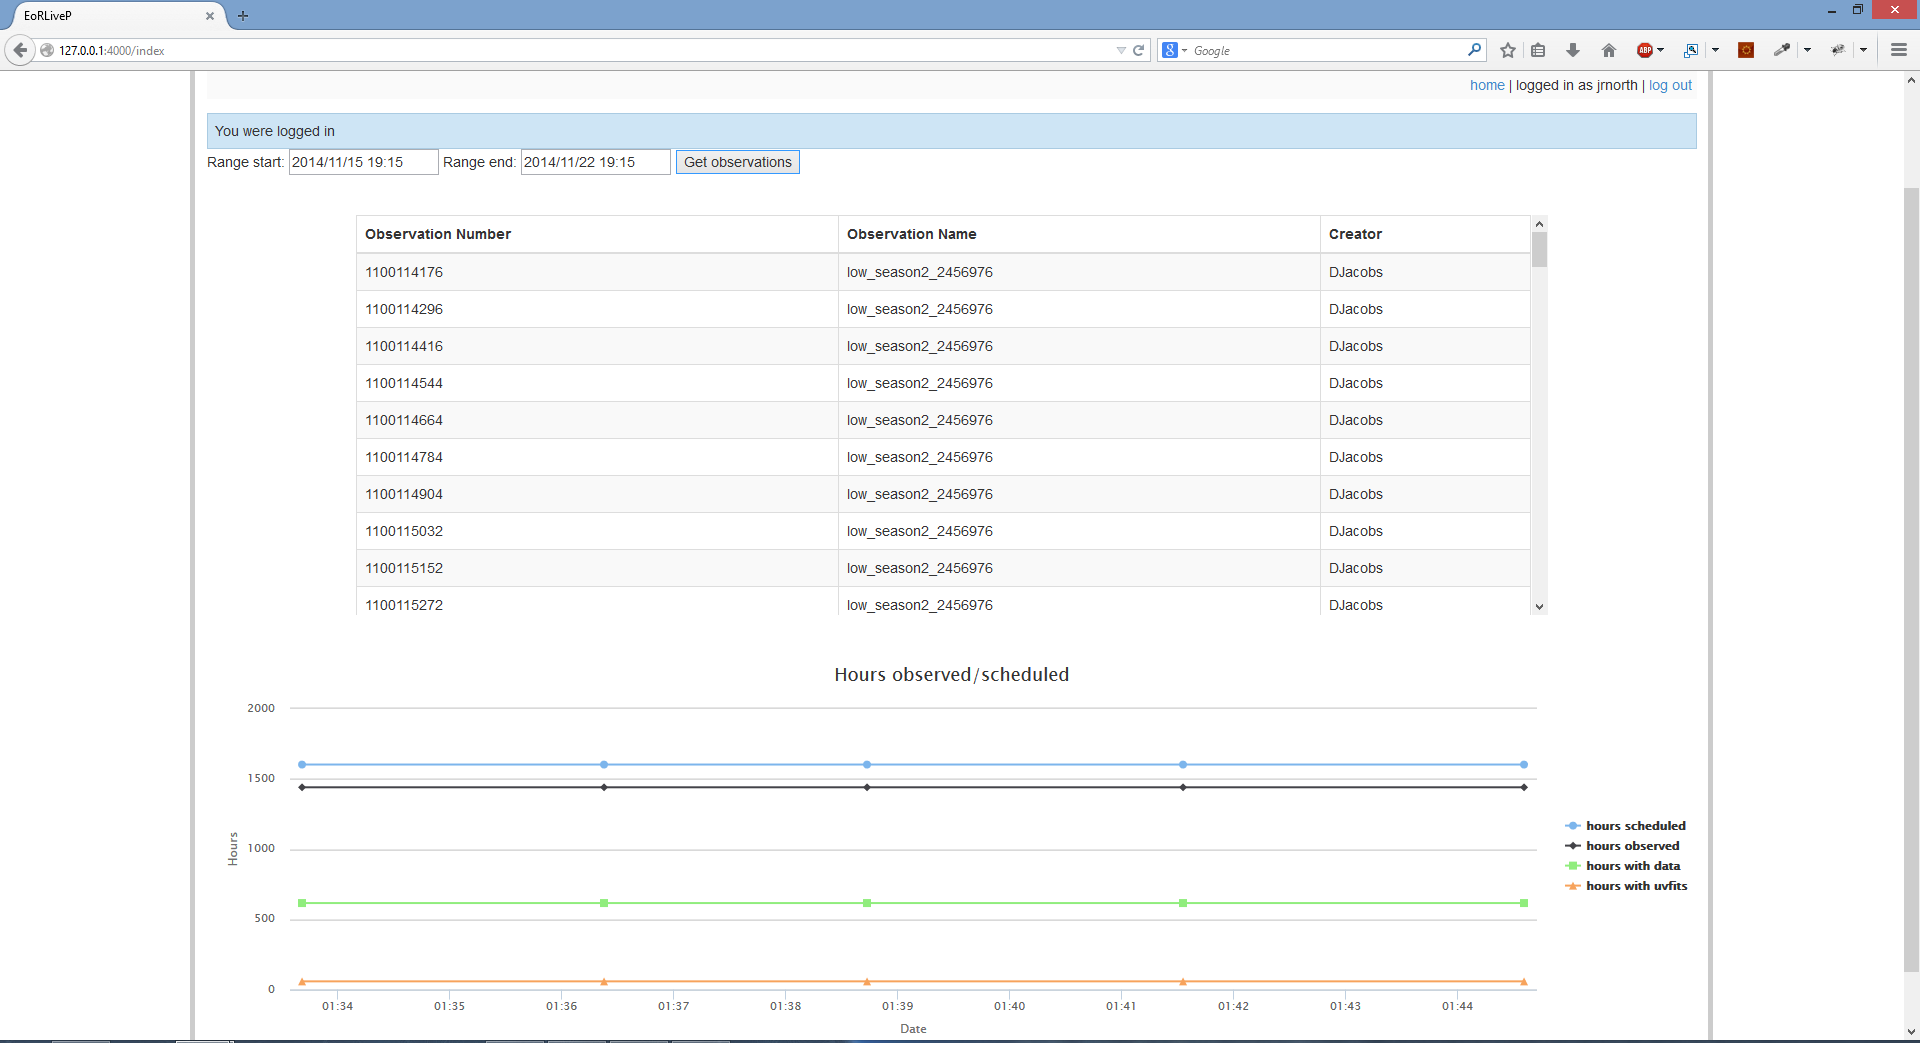
\includegraphics[width=\textwidth]{screenshot2}
\section{Problems and Risks}
One potential problem our sponsor pointed out to us early on is that the queries we would need to make on the MIT database have the potential to place an enormous load on the server. We needed to consider these performance concerns when designing our application. Our sponsor pointed us to a RESTful API maintained by the team that takes care of the database which places a smaller load on the server but only offers certain queries. We've had to figure out how to design our application using these Web services as much as possible so we can avoid using direct database queries.
\clearpage
\section{Summary of Tasks}

\subsection{Connor Alfheim}
\subsubsection{Team Presentation}
Connor prepared  and presented on the Design Overview content of the team presentation. He also offered suggestions for the lessons learned and tools section of the presentation during a mock team presentation. 
\subsubsection{Report}
Connor was the primary contributor to the Development Approach and the Design Overview section of the report. He also helped edit and proofread the rest of the report.
\subsubsection{Product}
Connor aided in the design of the database for the prototype. He helped identify and narrow down the key elements of the site to be first implemented. He also actively participated in the initial development of the design and structure of the prototype.
\subsubsection{Initialization Document}
Connor helped proofread the Initialization Document and offered content suggestions. 
\subsubsection{Team Management}
Connor helped with team management by steering team meetings to the appropriate subjects and keeping the meetings on track. Connor made sure the proper topics at each meeting were addressed concisely and adequately.

\clearpage

\subsection{Ryan Dougherty}
\subsubsection{Team Presentation}
Ryan created the shareable Google Drive link for the presentation. Also, in addition to filling out my slides for the section in which he presented, Ryan also gave some feedback to the rest of the team on their slides. Also, when the entire team met to test how much time our presentation took in total, Ryan took account of time for each individual, such as who needed to talk more, who needed to talk less, and other suggestions.
\subsubsection{Report}
Ryan created the initial document that was shared among our group. He also contributed some ideas among the group as to what to include in the final report, such as how much detail was needed to include in sections of the report. Also, he helped review some of the sections that were written by the other group members, by fixing grammar errors, including more details, and fixing flow between paragraphs and separate sections. In addition, Ryan also wrote Sections \#9 and \#10.
\subsubsection{Product}
Ryan was mainly the ``tester" of the group. As soon as a commit was made to the code repository, Ryan would pull the changes down from it and start up the virtual machine. If there were any problems with regard to features/usability that was seen in that pull, Ryan would create an issue/feature request on our repository on GitHub. After that, Ryan would then communicate with the rest of the team as to specifics of the issue/feature.
\subsubsection{Initialization Document}
Ryan, like in the team presentation, gave feedback on each other's work in the initialization document. 
\subsubsection{Team Management}
Ryan helped team management by being helpful to the team in terms of being able to understand what is needed to move forward in the project, particularly in testing each version of (and commit to) the shared code repository. 

\clearpage

\subsection{David Ganey}
\subsubsection{Team Presentation}
David contributed to the team presentation by completing the relevant slides. Additionally, he contributed to discussion in a team meeting before the presentation date. David was able to present his material succinctly within the unexpected time constraint at the end of the presentation, while maintaining clarity and making our goals for the next semester clear.
\subsubsection{Report}
David contributed much of the content to the final report. He set up the \LaTeX\ skeleton (including the sections and table of contents) before beginning to write the executive summary, user stories, and use-case sections. He was also the primary contributor to the lessons learned, future work, and second semester components.
\subsubsection{Product}
David contributed to the development of the product in several ways. By taking detailed notes and asking questions at meetings with sponsors, he was able to identify a list of defined requirements to be implemented. He also assisted with troubleshooting the initial setup of the development environment. David also made a significant effort to review all code pushed, and to monitor the status of the repository to prevent issues with the version control.
\subsubsection{Initialization Document}
David contributed significantly to the initialization document. He created and added the use-case diagrams to the \LaTeX\ document. He also edited the introduction, description, and milestones sections. He rewrote the user stories for resubmission of the document. Additionally, David promoted the feature-branch workflow by setting up a Git branch for the initialization document. He made other miscellaneous fixes to tables and formatting as necessary.
\subsubsection{Team Management}
David helped manage the team by being a point of contact between the team and the project sponsors. He frequently sent emails to the entire group to set up meetings and keep track of progress. As mentioned above, David also assisted with source code management by defining the Git workflow.

\clearpage

\subsection{Dylan Lusi}
\subsubsection{Team Presentation}
Dylan contributed to the team presentation by completing the technology decisions and rationale slides.  Also, he was able to effectively and clearly present the material before the class within two minutes by memorizing a script he had written.
\subsubsection{Report}
Dylan contributed to the team report by adding information to the 'Technology' section of the report.  He also reviewed the entire rough draft of the report for potential grammatical errors and missing information.
\subsubsection{Product}
Dylan contributed to the product by paying careful attention to the requirements of the sponsors during meetings and reviewing code in the GitHub repo for potential errors.
\subsubsection{Initialization Document}
Dylan contributed by reviewing the rough draft for potential errors, and giving feedback. 
\subsubsection{Team Management}
Dylan deferred to the superior management of his teammates.  He facilitated their management by attending, on time, every group meeting.

\clearpage

\subsection{Joseph North}
\subsubsection{Team Presentation}
Joseph contributed to the team presentation by producing and presenting the content in the Results section, including the video demonstrating the team's progress.
\subsubsection{Report}
Joseph wrote the preliminary results, problems and risks, and project description and motivation sections. He also made significant edits to the first draft of the report, including grammar and spelling fixes as well as adjusting the content as necessary.
\subsubsection{Product}
Joseph implemented the prototype, the primary project deliverable for the semester. He implemented the Vagrant virtual machine configuration, databases, and the backend and frontend layers of the site. Additionally, he produced documentation explaining the prototype's structure and how to get it up and running.
\subsubsection{Initialization Document}
Joseph wrote the introduction and conclusion sections of the project initialization document, and assisted in reformatting the user stories into the correct format prior to the document's resubmission.
\subsubsection{Team Management}
Joseph improved the team's communication by recognizing that Facebook was lacking as a collaboration tool and getting the team set up on Slack. He managed the prototype development by putting together a requirements document and getting feedback on it from the project sponsors. Additionally, he kept the team up-to-date by writing up the weekly meeting summaries and action items and posting them to the team's website.

\clearpage

\subsection{Ben Roos}
\subsubsection{Team Presentation}
Ben contributed to the team presentation by completing the PowerPoint slides covering the project background and motivation and presenting over the corresponding content. He also contributed to discussion and planning in a team meeting and rehearsal prior to the presentation.
\subsubsection{Report}
Ben contributed to the semester report by adding initial content to the first semester and success so far sections, by collaborating with others and discussing content for the project description and preliminary results sections, and by proof-reading others' contributions.
\subsubsection{Product}
Ben contributed to the development of the product by participating in team discussions to determine the requirements and core features of the product, by troubleshooting the development environment as it was set up and modified, by testing the prototype as development progressed, by discussing outstanding issues with other team members, and by reviewing code that was pushed to the shared repository.
\subsubsection{Initialization Document}
Ben contributed to the initialization document by proofreading its content, by providing feedback to other team members, and by assisting in finalizing its content.
\subsubsection{Team Management}
Ben contributed to team management by participating in all team meetings to determine features, design, and requirements, by maintaining continual communication with team members using Slack, and by discussing and clarifying the Git workflow with others.

\clearpage

\section{Conclusions}
\subsection{Success So Far}
Our work on the project thus far has culminated in a prototype of the EoRLive website in which users can log in, select a date range, and see the telescope observations and status of the telescope's data pipeline in that range. This prototype demonstrates some of the features that we set out to implement in our first semester and involves all three layers we laid out in our modified project scope. It will be a base on which we can add features to version 3 of the EoRLive website.
\subsection{Lessons Learned}
One of the primary lessons we learned was the difficulty of getting a project of this magnitude off the ground. While we consider ourselves a talented development team, it took a significant amount of time to identify the requirements, set up our development tools, and finally begin to create the product. We learned how difficult gathering requirements can be, in particular when gathering those requirements from users. Our sponsor suggested beginning with a prototype, which was very helpful. This allowed us to begin working quickly, without all the necessary pieces in place. In addition to learning the difficulty of beginning work, we learned how successful a prototype can be in jump-starting a development effort.
\subsection{Future Work}
As explained earlier, we have big plans for the second-semester development effort. The goal of the team is to create a fully re-engineered version three of the website (currently on its second iteration). By adding these features to the full website, the team hopes to enhance the scientists' research capabilities and leave the door open for easy modification of the website in the future.

\end{spacing}
\end{document}

